\documentclass[10pt]{article}

\usepackage[letterpaper,margin=1in]{geometry}
\usepackage{fontspec}
\usepackage{kotex}
\setmainfont{NanumMyeongjo}
\setsansfont{Noto Sans CJK KR}
\setmainhangulfont{NanumMyeongjo}
\setsanshangulfont{Noto Sans CJK KR}
\usepackage{microtype}
\usepackage{graphicx}
\usepackage{booktabs}
\usepackage{tabularx}
\usepackage{array}
\usepackage{enumitem}
\usepackage{xcolor}
\usepackage{amsmath}
\usepackage[font=small,labelfont=bf]{caption}
\usepackage{float}
\usepackage{tikz}
\usetikzlibrary{arrows.meta,positioning,fit,calc}
\usepackage{pgfplots}
\usepackage{pgfplotstable}
\pgfplotsset{compat=1.18}
\usepackage{url}
\usepackage[hidelinks]{hyperref}
\usepackage{cite}

\hypersetup{
  pdftitle={이 커밋을 승인한 주체는 누구인가? PAPER와 거버넌스 내재형 AI 통신},
  pdfauthor={Patrick Rho},
  pdfsubject={거버넌스 내재형 프로토콜 설계와 예비 프로토타입 평가},
  pdfkeywords={AI 거버넌스, 프로비넌스, 코딩 에이전트, 프로토콜, 역량 기반 보안}
}

\linespread{1.08}
\setlist{leftmargin=*,topsep=4pt,itemsep=2pt,parsep=1pt,partopsep=1pt}
\setlength{\parindent}{0pt}
\setlength{\parskip}{5pt plus 1pt minus 1pt}
\setlength{\textfloatsep}{18pt plus 3pt minus 3pt}
\setlength{\floatsep}{14pt plus 2pt minus 2pt}
\renewcommand{\arraystretch}{1.25}
\definecolor{paperink}{HTML}{263746}
\definecolor{paperblue}{HTML}{DCE8F0}
\definecolor{paperblueedge}{HTML}{58758A}
\definecolor{paperamber}{HTML}{E2A23A}
\definecolor{paperamberlight}{HTML}{FFF1D6}
\definecolor{papergray}{HTML}{EEF1F3}
\newcolumntype{Y}{>{\raggedright\arraybackslash}X}
\newcommand{\papername}{PAPER}
\newcommand{\system}{PCCP}
\renewcommand{\abstractname}{초록}
\renewcommand{\figurename}{그림}
\renewcommand{\tablename}{표}
\renewcommand{\refname}{참고문헌}

\title{\textbf{이 커밋을 승인한 주체는 누구인가?}\\\large PAPER와 거버넌스 내재형 AI 통신}
\author{Patrick Rho\\Patty Research}
\date{2026년 8월}

\begin{document}
\maketitle

\begin{abstract}
AI 코딩 에이전트는 비공개 저장소를 읽고, 외부로 전송할 정보를 선택하며, 모델과 도구를 호출하고, 파일을 수정하여 커밋까지 생성한다. 그러나 커밋이 만들어진 뒤에는 오히려 가장 기본적인 질문, 즉 \emph{누가 이 결과를 발생시킬 권한을 부여받았는가}에 답하기 어렵다. 현행 시스템은 API 자격 증명, 게이트웨이 판단, 도구 로그, Git 이력에서 단편적인 정보를 복원할 수 있다. 반면 인간의 의도에서 모델 호출과 실행 가능한 부수 효과에 이르는 전체 경로가 동일한 범위의 권한 아래 있었음을 일관되게 입증하지는 못한다. 여기서 결여된 것은 또 하나의 로그가 아니라 권한을 내포한 교환 단위이다.

본 논문은 거버넌스를 AI 통신 자체의 구성 요소로 만드는 상태 기반 프로토콜 \papername{}(Patty AI Provenance \& Enforcement Relay)를 제안한다. 핵심 추상화인 Governed Exchange는 등록된 피어와 인간 사용자의 신원을 단기 Capability Lease, 불변 Policy Epoch, 인라인 Relay Verdict, 서버 권위형 모델 패키지 및 엔드포인트, 콘텐츠 주소형 Provenance Spine과 결합한다. 이에 따라 모델은 행위를 제안할 수 있으나 실행 권한을 스스로 만들어낼 수 없으며, 증거는 사후에 조립되는 대신 인과 경로를 따라 생성된다.

본 연구는 해당 설계의 보안 경계를 규정하고 Go 프로토타입의 예비 측정 결과를 제시한다. Apple M4 Pro 환경에서 1~KiB Record 인코딩/디코딩의 중앙값은 290.2~ns, 1~MiB에서는 97.0~$\mu$s였으며, 증거 체인 갱신은 73.05~ns, Ed25519 서명 및 검증은 42.7~$\mu$s였다. 이는 원시 연산 비용일 뿐 종단 간 성능 결과가 아니다. 운영 수준 인증, 정책 파이프라인 지연, TTFT, 확장성 및 프로비넌스 충실도는 후속 평가가 필요하다. 본 연구의 핵심 결론은 구조적이다. 에이전트가 지속적인 부수 효과를 일으킬 수 있다면, 권한과 인과 증거는 그 작업을 운반하는 프로토콜의 일급 속성이어야 한다.
\end{abstract}

\section{서론}

다음과 같은 사고를 가정한다. 개발자가 에이전트에게 실패한 권한 부여 테스트의 수정을 요청한다. 에이전트는 저장소 파일 여섯 개를 컨텍스트로 선택하고, ``Code Standard''라는 이름의 모델을 호출한 뒤 셸 도구 제안을 받아 마이그레이션을 실행한다. 이어 두 파일을 수정하고 커밋을 생성한다. 수 시간 후 이 마이그레이션이 테넌트 데이터를 노출했다는 사실이 드러난다. 이때 조직은 다음 질문에 답해야 한다.

\begin{itemize}
  \item 어떤 인간 사용자와 어떤 설치형 에이전트가 작업을 시작했는가?
  \item 해당 에이전트는 그 모델에 여섯 개 파일을 공개할 권한이 있었는가?
  \item 어느 불변 정책 버전이 마이그레이션 명령을 허용했는가?
  \item 모델은 명령을 제안했을 뿐인가, 아니면 권한을 부여받은 런타임이 이를 실행했는가?
  \item 어떤 모델 패키지와 서빙 엔드포인트가 제안을 생성했는가?
  \item 모델 출력 중 어느 부분이 인간의 수정 이후에도 최종 커밋에 남았는가?
\end{itemize}

각 구성 요소에는 로그가 존재할 수 있다. 바로 그 점이 문제이다. API 인증은 한 경계의 호출자를 식별하고, 게이트웨이는 다른 경계에서 라우팅 또는 정책 판단을 기록하며, 샌드박스는 실행을, Git은 결과 아티팩트를 기록한다. 조직은 서로 다른 식별자, 시계, 보존 정책, 신뢰 가정 아래 생성된 기록을 결합하여 하나의 인과 및 권한 부여 서사를 재구성해야 한다. 공백이나 모호성은 부수 효과가 이미 발생한 뒤에야 발견된다.

이는 본질적으로 관측성 문제가 아니라 \emph{프로토콜 모델의 문제}이다. 기존 AI 인터페이스는 프롬프트, 토큰, 도구 호출, 작업, 아티팩트를 전달하지만, 이들이 부수 효과를 일으킬 수 있는 제한된 권한을 실시간 교환에 포함하도록 요구하지 않는다. 그 결과 거버넌스는 교환의 진행 조건이 아니라 교환을 둘러싼 미들웨어가 된다.

\papername{}는 이 관계를 역전한다. 지능적 처리를 먼저 운반하고 사후에 권한을 복원하는 대신, 프로토콜은 지능적 처리를 \emph{권한을 내포한 봉투} 안에서 전달한다. TLS 연결이 존재하거나 모델이 도구 호출을 출력했다는 사실만으로 보호된 교환이 진행되지는 않는다. 관련 신원, 목적, Lease, Policy Epoch, 모델 해석, Relay 판단이 모두 일치해야 다음 상태로 전이할 수 있다. 그림~\ref{fig:overview}는 이러한 구조적 전환을 나타낸다.

\begin{figure*}[t]
  \centering
  
\includegraphics[width=0.96\textwidth]{figures/qwen-governed-exchange.png}
  \caption{구조적 역전. 기존 시스템은 상호작용을 먼저 전달한 뒤 로그에서 권한을 복원한다. PAPER는 제한된 권한, 집행, 모델 식별, 인과 증거를 실시간 경로의 진행 조건으로 둔다. 본 그림은 개념도이며 경험적 데이터를 포함하지 않는다.}
  \label{fig:overview}
\end{figure*}

\subsection{연구 기여}

본 논문의 주장은 하나이다. \emph{에이전트형 AI 프로토콜은 메시지와 행위뿐 아니라 그 행위를 정당화하는 권한 및 인과 증거를 함께 운반해야 한다.} 이를 뒷받침하는 기여는 다음 세 가지이다.

\begin{enumerate}
  \item \textbf{Governed Exchange.} 인간 및 피어 신원, 목적 한정 Capability Lease, 불변 Policy Epoch, 모델 권위, 인라인 Relay Verdict를 보호 행위의 선행 조건으로 삼는 프로토콜 수명주기를 정의한다. 모델의 제안은 데이터이며 실행 권한은 모델 외부에 존재한다.
  \item \textbf{인과적 권한 체인.} 사용자에게 보이는 모델 선택을 서명된 모델 패키지와 임대된 엔드포인트에 연결하고, 의도, 정보 공개, 추론, 도구 활동, 편집, 아티팩트를 콘텐츠 주소형 Provenance Spine 및 서명 영수증으로 결합한다. 목표는 더 많은 텔레메트리가 아니라 \emph{왜 이 부수 효과가 허용되었는가}에 대한 검증 가능한 답이다.
  \item \textbf{측정된 프로토타입 기반.} Go로 프레이밍, 정규 객체, 서명, 증거 체인, 전송 기반, 개발용 Relay--PIA 경로를 구현한다. 재현 가능한 원시 연산 비용과 프로토타입이 아직 입증하지 못한 범위를 함께 보고한다.
\end{enumerate}

신규성 주장은 의도적으로 조합적이다. 보안 전송, Capability, 프로비넌스 DAG, 서명 영수증, 도구 프로토콜은 이미 존재한다. PAPER의 주장은 이들의 권한 의미론이 Harness--Relay--추론/런타임 경계의 단일 실시간 상태 기계에 속해야 한다는 것이다. 이 명제가 성립한다면 거버넌스는 부수 효과 이전에 집행되고, 증거는 우연히 맞아떨어지는 포렌식 기록이 아니라 프로토콜 출력이 된다.

\section{결여된 계층}

앞의 사고 사례는 에이전트 시스템에서 반복되는 세 가지 불일치를 드러낸다.

\paragraph{인증은 권한 이력이 아니다.}
유효한 API 자격 증명은 요청을 시작한 주체를 식별할 수 있으나, 장시간 작업 전체에서 어떤 저장소, 목적, 도구 종류, 모델 아티팩트, 부수 효과가 허용되었는지는 확정하지 못한다. 에이전트 작업은 개별 요청보다 오래 지속되며, 상이한 권한 모델을 가진 여러 구성 요소를 통과한다.

\paragraph{모델 출력은 실행 권한이 아니다.}
도구 호출 형식은 제안된 행위를 기계 판독 가능하게 만들 뿐 정당하게 만들지는 않는다. 모델이 특정 구문을 출력했다는 이유로 실행이 가능하다면, 신뢰할 수 없는 저장소 텍스트는 프롬프트 인젝션을 통해 권한을 획득하려 할 수 있다. 따라서 집행 경계는 제안, 승인, 실행을 서로 다른 주체가 담당하는 별개의 사건으로 구분해야 한다.

\paragraph{로그는 사건을 기록하지만 단일 인과 경로를 반드시 입증하지는 않는다.}
상관 식별자는 유용하지만 상관관계가 프로토콜로 강제된 체인과 동일하지는 않다. ``누가 이 커밋을 승인했는가''에 대한 지속 가능한 답은 실행 전에 존재했던 권한 및 정책에 행위를 결합하고, 이후 인간과 자동화 작업을 거치며 결과가 어떻게 변했는지 보존해야 한다.

따라서 보안 전송과 응용별 거버넌스 사이에는 신원, 제한된 권한, 불변 정책, 집행 판단, 증거를 조정된 프로토콜 상태로 운반하는 교환 계층이 필요하다.

\section{인접 시스템과 신규성의 경계}

\paragraph{모델 API와 게이트웨이.}
HTTPS/JSON 및 스트리밍 모델 API는 효과적인 요청/응답 인터페이스이며, 게이트웨이는 인증, 할당량, 정책, 로깅을 추가할 수 있다. PAPER의 주된 차이는 상태의 단위이다. 권한과 증거를 독립적인 미들웨어 사건에서 사후 복원하지 않고 장기 거버넌스 세션 및 교환에 결합한다.

\paragraph{MCP와 A2A.}
Model Context Protocol(MCP)은 AI 응용과 컨텍스트/도구 제공자 간 상호작용을 표준화한다~\cite{mcp2025}. Agent2Agent(A2A)는 에이전트 탐색, 작업, 메시지, 아티팩트를 표준화한다~\cite{a2a2026}. PAPER는 이들을 열등한 전송 방식으로 보지 않는다. MCP는 거버넌스형 도구 브로커 뒤에 배치될 수 있고 A2A는 에이전트 간 경계에서 동작할 수 있다. PAPER는 인간 대상 엔지니어링 Harness, 인라인 정책 집행, 통제된 추론/런타임 인프라, 소프트웨어 프로비넌스 사이의 더 좁은 경계를 다룬다.

\paragraph{런타임 거버넌스와 에이전트 보안.}
MI9은 에이전트 시스템의 통합 런타임 거버넌스를 연구하고~\cite{wang2025mi9}, AgentDojo는 프롬프트 인젝션 공격 및 방어 환경을 제공하며~\cite{debenedetti2024agentdojo}, 인자 수준 프로비넌스 연구는 거친 권한 부여와 도구 인자 사이의 불일치를 지적한다~\cite{fan2026granularity}. PAPER는 이에 상보적이며, 신원, 정책, 도구 권한, 증거를 집행하고 반출할 수 있는 프로토콜 객체와 상태 전이를 정의한다.

\paragraph{공급망 프로비넌스.}
in-toto는 공급망 단계의 서명 메타데이터를 기록하고~\cite{torresarias2019intoto,intoto}, SLSA는 빌드 및 소스 트랙의 프로비넌스 기대 수준을 정의한다~\cite{slsa12}. SCITT는 디지털 아티팩트에 관한 서명 진술을 등록하고 영수증을 발급하는 투명성 서비스를 정의한다~\cite{rfc9943}. PAPER는 빌드 아티팩트가 생기기 전의 상호작용 단계에서 컨텍스트, 추론, 부수 효과의 허용 여부를 통제한다. PAPER 영수증은 이후 in-toto/SLSA 증명 입력이나 SCITT 진술이 될 수 있지만, 아티팩트 투명성이 실시간 교환 권한을 대체하지는 않는다.

\paragraph{신원 및 암호학적 구성 요소.}
SPIFFE는 워크로드 신원 규약을 제공한다~\cite{spiffe}. PAPER는 TLS~1.3~\cite{rfc9846}, QUIC~\cite{rfc9000}, 결정적 CBOR~\cite{rfc8949}, COSE~\cite{rfc9052}, HPKE~\cite{rfc9180}, COSE 영수증~\cite{rfc9942}을 재사용한다. 이 표준들은 전송 및 객체 보안의 기반을 제공하지만 본 연구가 제안하는 응용 수준 권한 모델을 정의하지는 않는다.

신규성의 경계는 다음과 같이 요약된다. MCP는 도구를 기술하고, A2A는 에이전트 간 작업을 기술하며, SPIFFE는 워크로드를 식별하고, 게이트웨이는 정책을 집행하며, in-toto는 공급망 단계를 증명할 수 있다. PAPER는 AI 엔지니어링 행위가 계산 제안에서 권한 있는 지속적 부수 효과로 넘어가는 시점에 이 요소들을 하나의 거버넌스 상태 기계로 결합할 수 있는지를 묻는다.

\section{요구사항과 위협 모델}

\subsection{설계 요구사항}

사고 사례의 질문은 여섯 가지 요구사항으로 변환된다. (R1) 모든 보호 행위를 등록 피어 및 인간 신원에 결합한다. (R2) 단기·목적 한정 권한으로 권한 범위를 제한한다. (R3) 모든 집행 판단을 불변 정책 개정판에 결합한다. (R4) 호출자가 제공한 이름보다 강한 방식으로 서빙 모델 아티팩트와 엔드포인트를 식별한다. (R5) 모델 제안과 런타임의 승인 및 실행을 분리한다. (R6) 일반 응용 로그보다 오래 유지되는 인과 증거를 생성한다.

시스템은 제어 평면이 일시적으로 가용하지 않은 상황에서도 동작해야 한다. 따라서 Relay는 서명 또는 인증된 스냅샷, 폐기 상태, Policy Epoch, 모델 카탈로그, Lease를 소비한다. 오래된 상태를 사용할 수 있는 범위는 암묵적 캐시 동작이 아니라 명시적 만료 및 배포 정책으로 제한한다.

\subsection{공격자와 비목표}

네트워크 공격자, 미등록 클라이언트, 탈취·재생된 자격 증명, 침해된 Harness, 프롬프트 인젝션 콘텐츠, 악성 도구 출력, 모델명 위조, 테넌트 간 오조작, 증거 변조를 고려한다. Relay 또는 관리자 역시 악의적이거나 침해될 수 있다. 프로토콜은 권한과 증거의 경계를 명시하는 것을 목표로 하지만, 평문을 처리하는 신뢰 Relay의 열람을 막거나 모델의 올바른 행동을 증명하거나 완전히 침해된 엔드포인트의 프로토콜 외부 행위를 막지는 못한다. 하드웨어 증명과 형식 검증은 선택 가능한 후속 프로파일이며 현재 프로토타입의 가정이 아니다.

\section{Governed Exchange}

Governed Exchange는 PAPER에서 책임 추적이 가능한 AI 작업의 단위이다. API 요청보다는 크고 전체 개발자 세션보다는 작다. Harness가 보호 목적을 선언할 때 시작하여 결과 증거를 확정하는 영수증으로 종료한다. 이 경계 안에서 추론, 컨텍스트 공개, 모델 선택, 도구 사용, 승인, 출력은 권한 인지형 상태 기계의 전이로 표현된다.

이를 데이터베이스 일관성이 아니라 거버넌스를 커밋 조건으로 삼는 트랜잭션으로 볼 수 있다. TLS는 바이트가 보호된 채널을 통해 전달되었는지를 답한다. Governed Exchange는 발신자, 목적, 정책, 모델, 제안된 부수 효과가 서로 일치하는지까지 확인한다. 필수 게이트를 통과하지 못하면 보호 전이가 차단되며, 사후 로그만 남기는 것으로 대체하지 않는다.

\subsection{아키텍처와 피어}

관리 Control Plane은 신원을 등록하고 정책 및 모델 상태를 발급하며, 폐기 상태를 관리하고 증거를 색인한다. 권위는 갖지만 모든 토큰 경로에 동기식으로 배치되지는 않는다. Relay는 Harness 연결을 종단하고 캐시된 서명 상태를 검증하며, 인라인 정책 판단, 승인된 추론 라우팅, 증거 추가를 수행한다. Patty Inference Agent(PIA)는 서빙 엔진 앞에 위치한 등록 피어이다. PIA는 PAPER의 의미 요청을 로컬 엔진 인터페이스로 변환하며, 원시 모델 엔드포인트는 Harness의 라우팅 권위가 될 수 없다. 런타임은 독립적인 권한 전이가 완료된 뒤에만 도구를 실행한다.

\begin{table*}[t]
\centering
\caption{핵심 권한 및 신원 객체. Harness에 노출되는 객체와 배포 신원을 의도적으로 분리한다.}
\label{tab:objects}
\small
\begin{tabularx}{\textwidth}{@{}l l Y Y@{}}
\toprule
객체 & 발급 권위 & 목적 & 핵심 구분 \\
\midrule
Peer credential & 등록 권위 & 키, 피어 프로파일, 테넌트, 유효기간 결합 & 사용자뿐 아니라 소프트웨어 인스턴스 식별 \\
Capability Lease & 정책 권위 & 행위·모델·도구·컨텍스트 범위의 제한적 부여 & 자원 용량이 아니라 행위 권한 \\
Policy Epoch & 정책 권위 & 유효 정책의 불변 개정판 & ``최신''이 아니라 다이제스트에 결합 \\
Catalog Model & 모델 카탈로그 & 사용자에게 보이는 안정적 서비스 신원 & 제공자 엔드포인트를 포함하지 않음 \\
Model Descriptor & 모델 카탈로그 & 의미 기능 및 최소 클라이언트 요건 선언 & 협상 정보이며 그 자체가 권한은 아님 \\
Model Package (PMP) & 모델 권위 & 서명된 아티팩트·템플릿·양자화 신원 & 사람이 읽는 모델명보다 강한 식별 \\
Endpoint Lease & 서빙 권위 & 활성 PIA 엔드포인트와 승인 패키지 결합 & 단기 배포 상태 \\
Account Capacity Lease & 용량 권위 & 분산 워크로드 슬롯 조정 & 행위 권한과 구별되는 용량 \\
\bottomrule
\end{tabularx}
\end{table*}

\subsection{확장된 로그 스키마가 아니라 프로토콜인 이유}

로그 스키마는 허용 판단을 기술할 수 있으나, 정보 공개, 모델 할당, 도구 실행보다 먼저 판단이 이루어지도록 강제할 수는 없다. 상태 기계형 프로토콜은 이를 강제할 수 있다. PAPER는 신원 결합, Lease 제시, Epoch 결합, Verdict, 디스패치, 도구 승인, 종료를 피어가 순서대로 완료해야 하는 관측 가능한 전이로 만든다. 이 순서성이 거버넌스 인지형 미들웨어와 거버넌스 내재형 통신을 구분한다.

교환 $x$에서 시각 $t$에 보호 행위 $a$가 시도된다고 하자. PAPER는 다음 조건이 성립할 때에만 해당 상태 전이를 허용한다.

\begin{equation}
\operatorname{advance}(x,a,t) = P_x \land S_x \land L_x(a,t)
  \land E_x \land V_x(a) \land R_x(a),
\label{eq:advance}
\end{equation}

여기서 $P_x$와 $S_x$는 유효한 피어 및 세션 결합, $L_x(a,t)$는 행위 $a$를 포함하는 만료 전 Capability Lease, $E_x$는 인식된 불변 Policy Epoch, $V_x(a)$는 허용 Relay Verdict를 뜻한다. $R_x(a)$는 행위별 권한을 모은다. 추론에는 승인된 모델 패키지와 유효한 Endpoint Lease가, 부수 효과에는 독립적인 도구 권한이 필요하다. 식~\ref{eq:advance}는 프로토콜 수락 조건이며 형식적 보안 증명이 아니다. 어느 한 항이라도 거짓이면 보호 전이는 차단된다.

\subsection{전송과 표현}

독립 스트림이 head-of-line 결합을 줄이므로 QUIC을 우선 바인딩으로 사용하며 TLS~1.3 over TCP를 대체 경로로 둔다. 두 전송은 동일한 응용 의미론과 ALPN 신원을 사용한다. Record는 고정 prelude, 정규 헤더, payload, 논리 lane 식별자, lane sequence를 포함한다. 결정적 CBOR은 재현 가능한 객체 인코딩을 제공하고, 객체 수준 검증이 필요한 자격 증명, Lease, Epoch, 모델 manifest, 영수증은 COSE 서명으로 보호한다.

전송 인증만으로는 충분하지 않다. 응용 증명은 피어 자격 증명, nonce, 협상 프로파일, 채널 문맥을 결합하여 한 연결에서 캡처한 증명을 다른 연결에서 재생하지 못하게 해야 한다. 현재 프로토타입은 이 메시지를 정의하지만, 절~\ref{sec:implementation}에서 설명하듯 운영 수준의 전체 검증 경로를 아직 수행하지 않는다.

\section{교환이 다음 상태로 진행할 권리를 얻는 방법}

\subsection{신원, 세션, Capability Lease}

사용자 신원, Harness 신원, 워크로드/세션 신원은 각각 누가 작업을 요청했는지, 어떤 소프트웨어 설치가 이를 전달했는지, 현재 어떤 제한된 활동이 진행 중인지를 답하므로 분리한다. 등록은 Harness에 피어 자격 증명을 부여할 뿐 추론 또는 도구 권한을 주지 않는다. Working Session은 사용자, Harness, 조직/프로젝트, 목적, 저장소, 유효 정책을 결합한다. Capability Lease는 허용 모델, 컨텍스트 경로, 도구 종류, 토큰 예산, 승인 요건 등 행위의 부분집합을 짧은 기간 동안 부여한다. 전송 연결이 유지되더라도 폐기 또는 만료가 발생하면 새로운 보호 행위를 차단한다.

\subsection{Policy Epoch과 Relay Verdict}

Policy Epoch은 교환에서 ``허용됨''의 의미를 고정한다. 감사 시점의 최신 정책을 가리키는 포인터가 아니라 다이제스트로 주소화한 불변 스냅샷이다. 세션 중 정책이 바뀌면 활성 작업은 계속, 재결합, 일시정지, 종료 중 명시된 규칙을 따르며 과거의 의미가 자동으로 바뀌지 않는다. 보호 콘텐츠가 PIA나 런타임에 도달하기 전에 Relay는 허용, 거부, 변환, 격리, 승인 요구 등의 구조화된 Verdict를 발행하고, 판단에 사용한 Epoch과 규칙 집합을 명시한다.

\subsection{교환 수명주기}

일반적인 교환은 \textsc{open}, \textsc{governance}, \textsc{route}, \textsc{stream}, 선택적 \textsc{tool/approval}, \textsc{close} 순으로 진행한다. 이는 설명용 이름이 아니라 각 단계에서 합법적인 메시지를 제한하는 상태이다. Relay는 디스패치 전에 피어/세션 결합, Capability Lease, Policy Epoch, Catalog Model, Model Package, Endpoint Lease, 용량 상태를 검증한다. 토큰 또는 데이터 Record는 순번이 있는 lane으로 다중화한다. 부수 효과 행위에는 멱등성 등급을 부여하여 재연결 또는 재개가 완료된 동작을 중복 실행하지 못하게 한다.

앞의 사고 사례에 적용하면 답이 분명해진다. 여섯 파일은 Harness를 떠나기 전에 Lease와 Epoch에 따라 공개 여부가 결정된다. ``Code Standard''는 추론 전에 서명 패키지와 Lease가 있는 PIA 엔드포인트로 해석된다. 셸 문자열은 별도로 권한을 받은 런타임 전이가 실행할 때까지 제안으로 남는다. 최종 영수증은 이 판단들을 이후 커밋에 연결되는 증거 루트에 결합한다.

그림~\ref{fig:lifecycle}는 이 순서를 나타낸다. 도구가 제안되는지는 선택적이지만, 제안된 도구의 권한 부여는 선택 사항이 아니다.

\begin{figure}[H]
  \centering
  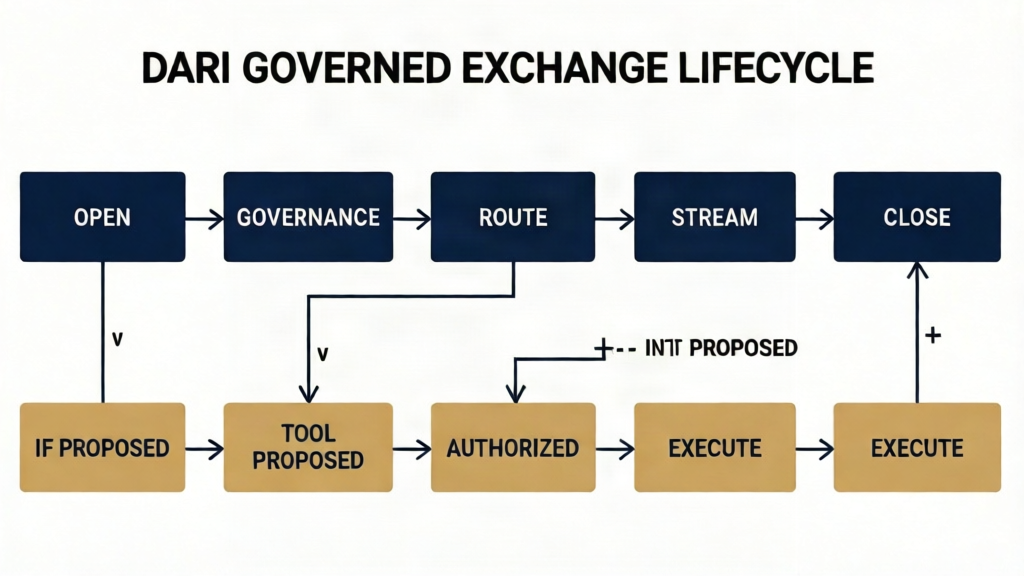
\includegraphics[width=\textwidth]{figures/governed-exchange-lifecycle.png}
  \caption{Governed Exchange의 프로토콜 설계. 보호 작업은 순차적 권한 게이트를 통과한다. 모델이 도구를 제안할 수는 있으나 실행 전에 독립적인 권한 전이가 반드시 필요하다. 본 그림은 의도한 의미론을 설명하며 구현 범위를 측정한 결과가 아니다.}
  \label{fig:lifecycle}
\end{figure}

\subsection{서버 권위형 모델 해석}

모델명은 사용자 경험을 위한 이름이지 보안 신원이 아니다. PAPER는 다음 세 식별자를 구분한다.

\begin{equation*}
\text{Catalog Model} \rightarrow \text{PMP} \rightarrow \text{PIA Endpoint}.
\end{equation*}

인증 후 Harness는 권리, 조직 정책, 배포 프로파일, 지역, 클라이언트 기능에 맞게 제한된 유효 모델 카탈로그를 받는다. Model Descriptor는 멀티모달 입력, 구조화 출력, 병렬 도구, 캐시, 추론 제어, 재개 가능성과 같은 의미 기능을 광고하되 엔드포인트를 공개하지 않는다. inference-open 메시지는 Catalog Model과 Catalog Epoch을 참조한다. Relay는 오래되거나 허용되지 않은 선택을 거부하고, 서명된 Patty Model Package(PMP)를 해석한 뒤 유효한 Lease가 있는 PIA 엔드포인트를 선택한다. Catalog Model은 사용자에게 보이는 안정적 제품 신원, PMP는 승인된 아티팩트 및 서빙 구성, Endpoint Lease는 해당 패키지가 현재 실행될 수 있는 위치를 뜻한다. 호출자는 선호를 표현할 수 있지만 문자열이나 base URL을 신뢰 인프라로 바꿀 수 없다.

그림~\ref{fig:model-identity}는 사용자에게 보이는 이름이 라우팅 권위가 되지 않도록 세 신원을 분리하는 방식을 보인다.

\begin{figure}[H]
  \centering
  \begin{tikzpicture}[
  font=\small,
  identity/.style={draw=paperblueedge, fill=paperblue, rounded corners=2pt,
    minimum width=2.65cm, minimum height=1.12cm, align=center,
    text=paperink, font=\small\bfseries},
  runtime/.style={draw=paperink, fill=papergray, rounded corners=2pt,
    minimum width=2.65cm, minimum height=1.12cm, align=center,
    text=paperink, font=\small\bfseries},
  resolve/.style={-{Latex[length=2.2mm]}, very thick, draw=paperink},
  local/.style={-{Latex[length=2.2mm]}, thick, dashed, draw=paperblueedge},
  kind/.style={font=\scriptsize, text=paperblueedge, align=center}
]
  \node[identity] (catalog) {Service Model};
  \node[identity, right=0.52cm of catalog] (manifest) {모델 아티팩트\\명세서};
  \node[identity, right=0.52cm of manifest] (grant) {인가 증서};
  \node[runtime, right=0.52cm of grant] (peer) {추론 피어};
  \node[runtime, right=0.52cm of peer] (engine) {서빙 엔진};

  \node[kind, below=0.16cm of catalog] {제품 식별자\\사용자에게 표시};
  \node[kind, below=0.16cm of manifest] {아티팩트 식별자\\서명된 구성};
  \node[kind, below=0.16cm of grant] {제한적 권한\\대상과 범위};
  \node[kind, below=0.16cm of peer] {배포 식별자\\라우팅 대상};
  \node[kind, below=0.16cm of engine] {로컬 어댑터\\응용에 비공개};

  \draw[resolve] (catalog) -- (manifest);
  \draw[resolve] (manifest) -- (grant);
  \draw[resolve] (grant) -- (peer);
  \draw[local] (peer) -- (engine);
\end{tikzpicture}

  \caption{서버 권위형 모델 해석. 제품, 아티팩트, 배포 신원은 Relay가 등록 PIA로 해석할 때까지 구분된다. 서빙 엔진은 로컬 구현 세부사항이며 Harness가 선택할 수 있는 엔드포인트가 아니다.}
  \label{fig:model-identity}
\end{figure}

\subsection{도구 권한과 프롬프트 인젝션}

PAPER의 핵심 프롬프트 인젝션 규칙은 한 문장으로 요약된다. \emph{모델 출력은 제안이지 권한이 아니다.} Tool Descriptor는 실행 위치, 위험 등급, 인자 스키마, 승인 정책, 멱등성, 프로비넌스 요건을 지정한다. 스트리밍 중인 인자는 완전한 형태로 수신되고 권한이 확인되기 전까지 실행할 수 없다. 저장소 텍스트, 채팅, 파일, 도구 출력은 신뢰 레이블을 유지하지만 Lease 범위를 확장할 수 없다. 프롬프트 인젝션 자체는 여전히 가능하나, 주입된 텍스트는 자신이 통제하지 못하는 권한 경계를 넘어야 한다. PAPER는 제안과 그 실행을 허용·변환·거부한 독립 판단을 모두 기록한다.

\section{인과 프로비넌스와 영수증}

가장 강한 감사 질문은 ``어떤 사건이 있었는가''가 아니라 ``어떤 권한 아래 무엇이 이 아티팩트의 생성을 야기했는가''이다. Provenance Spine은 인간의 의도, 선택한 컨텍스트, 정책 판단, 모델 호출, 출력, 도구 제안, 승인, 실행 결과, 편집, 테스트, 검토, 소스 제어 아티팩트 사이의 인과 간선을 표현한다. 노드는 콘텐츠 주소와 유형을 가지며 간선은 원인, 파생, 공개, 변환, 결합을 기술한다. 프로토콜이 요구하는 전이가 누락되면 서로 무관한 로그의 한 행이 빠진 것이 아니라 인과 설명에 검증 가능한 공백이 남는다. PAPER는 거버넌스 경로 밖에서 완전히 수행된 사건을 영수증이 드러낼 수 있다고 주장하지 않는다.

교환 무결성을 간결하게 표현하기 위해 $r_0=H(\textsf{domain}\parallel\textsf{exchange-open})$으로 두고 다음과 같이 정의한다.

\begin{equation}
r_i = H(\textsf{domain}\parallel r_{i-1}\parallel H(e_i)),
\end{equation}

$e_i$는 $i$번째 증거 사건의 정규 표현이다. 서명된 Evidence Receipt는 최종 루트를 교환, 신원, Policy Epoch, 모델/패키지 해석, 결과, 보존/반출 프로파일에 결합한다. 전체 순서 사건열을 가진 감사자는 루트를 다시 계산하여 종료된 교환과의 일관성을 검증할 수 있다. 임의의 선택 공개 부분집합을 증명하려면 별도의 commitment 또는 inclusion proof가 필요하며 현재 체인 원시 연산만으로는 제공되지 않는다.

이 구조는 변조 증거를 제공할 뿐 사실을 자동으로 보장하지 않는다. 침해된 권한 구성 요소는 거짓 원천 데이터를 낼 수 있고, 모든 서명자를 통제하는 공모 집단은 일관된 허위 기록을 만들 수 있다. 구성 요소 간 영수증과 외부 투명성은 단일 주체에 대한 신뢰를 줄이지만 제거하지는 않는다. ``암호학적으로 서명됨''과 ``사실임''은 다르다. PAPER는 명시된 구성 요소 가정 아래 전자를 주장하며 후자를 주장하지 않는다.

선택적 반출 프로파일은 민감한 노드를 commitment 또는 비식별 요약으로 대체할 수 있으나, 검증 가능한 연결은 현재 체인 벤치마크가 입증한 성질이 아니라 설계 요구사항이다. 리팩터링이나 병합 이후의 소스 코드 귀속은 확률적으로 다루고, 이진 ``AI 생성'' 레이블 대신 신뢰도와 변환 이력을 제시해야 한다.

\section{설계에서 실행 가능한 교환으로}
\label{sec:implementation}

설계가 도식에 머물지 않고 실행 가능한 프로토콜이 될 수 있는지 확인하기 위해 Go 프로토타입을 구현하였다. 평가 스냅샷은 저장소 커밋 \texttt{0234034}이다. 32바이트 Record prelude, 제한된 헤더와 payload, 정규 CBOR 도우미, COSE Sign1, Ed25519 객체 서명, 콘텐츠 주소형 다이제스트, 증거 체인 원시 연산, 피어/세션 상태 기계, TLS/TCP 전송, QUIC 전송 기반, 모델/카탈로그 스키마, 정책 및 Lease 서비스, Relay/PIA 구성 요소, vLLM/SGLang 어댑터, 적합성 테스트를 포함한다.

현재 수직 경로는 PAPER TLS/TCP 연결에서 \texttt{AI\_OPEN} 및 \texttt{AI\_COMPLETE} Record를 사용하여 Relay의 추론 요청을 PIA로 전달한다. PIA는 요청을 모델 서빙 어댑터로 변환하고 응답을 정규화한다. 이는 Harness 대상 경로가 사용자가 제공한 모델 엔드포인트가 아니라 등록된 프로토콜 피어에서 종료된다는 신뢰 배치를 입증한다.

그러나 아직 설계의 가장 강한 형태를 구현한 것은 아니다. 내장 AI 의미 payload는 최종 정규 인코딩이 아니라 JSON이며, PAPER PIA 주소가 없을 때 기존 HTTP 개발 fallback이 남아 있다. Listener는 완전한 COSE 서명, 폐기, 인증서, transcript 검증 없이 개발용 증명 자료를 수용한다. 한 카탈로그 경로는 유효 카탈로그가 아니라 존재 여부만 검사하고, 용량/스케줄러 게이트에는 허용적 stub이 있다. 표~\ref{tab:claims}는 이 경계를 명시한다. 불완전한 집행은 감출 각주가 아니라 프로토타입 성숙도에 관한 평가 결과로 취급한다.

\begin{table*}[t]
\centering
\caption{평가 프로토타입의 증거 경계. ``부분''은 관련 코드가 있으나 진술한 속성이 종단 간으로 완전히 시험되지 않았음을 뜻한다.}
\label{tab:claims}
\small
\begin{tabularx}{\textwidth}{@{}Y l Y Y@{}}
\toprule
메커니즘 또는 속성 & 상태 & 시험 내용 & 증거가 확립하는 범위 \\
\midrule
Record 프레이밍과 제한 파싱 & 구현 & 왕복 테스트와 마이크로벤치마크 & 원시 비용과 파서 동작 \\
정규 CBOR 및 서명 원시 연산 & 구현 & 단위 테스트와 마이크로벤치마크 & 원시 연산의 정확성과 비용 \\
변조 감지형 증거 체인 갱신 & 원시 연산 구현 & 결정적 변이 테스트와 마이크로벤치마크 & 명시된 해시 가정 아래 변이가 루트를 변경 \\
TLS/TCP Relay--PIA PAPER 교환 & 부분 & 구현 및 패키지 테스트 & 개발용 수직 경로의 실행 \\
인증된 Harness--Relay 교환 & 부분 & 메시지/상태 테스트, 증명 검증 미완료 & 메시지 수명주기이며 운영 인증은 아님 \\
Catalog Model 권한 부여 & 부분 & 스키마/서비스 테스트, 허용적 파이프라인 & 권한 모델은 인코딩됐으나 종단 간 폐쇄되지 않음 \\
계정 단위 분산 용량 집행 & 설계/골격 & 스키마와 서비스 골격 & 집행 결과 없음 \\
연구 불변조건 집행 & 미확립 & 이름이 있는 테스트 11개, 일부는 약하거나 placeholder & 후보 테스트 집합이며 12개 속성의 증명은 아님 \\
운영 지연, TTFT, 확장성, 프로비넌스 충실도 & 미측정 & 방법론만 정의 & 시스템 수준 결과 없음 \\
\bottomrule
\end{tabularx}
\end{table*}

\section{평가: PAPER가 유의미하기 위한 조건}

거버넌스 내재형 프로토콜은 상호작용형 AI를 사용할 수 없게 만들지 않으면서 권한을 실질적으로 더 잘 집행할 때에만 유용하다. 이에 따라 다음 질문을 설정한다. (Q1) PAPER가 연결 및 추론 전 지연에 추가하는 비용은 얼마인가? (Q2) 스트림 증가에 따라 Relay 비용은 어떻게 변하는가? (Q3) 검증 가능한 인과 경로를 위해 어느 정도의 증거 및 저장 비용을 지불하는가? (Q4) 관례가 아니라 프로토콜 상태가 거부하는 적대 사례는 무엇인가? (Q5) 실제 소프트웨어 변경 이후 프로비넌스는 얼마나 정확하게 유지되는가?

\subsection{기준선}

목표에 맞춘 다섯 기준선을 정의한다. B0는 최소 보안 이진 스트림, B1은 bearer 인증 HTTPS/JSON 스트리밍, B2는 동등한 게이트웨이 정책 및 로깅을 더한 HTTPS/JSON, B3는 신원/세션 및 최소 거버넌스를 적용한 PAPER, B4는 Lease, 정책, 콘텐츠 검사, Verdict, 프로비넌스를 적용한 PAPER이다. 핵심 비교는 동등한 거버넌스와 다른 수명주기를 비교하는 B2 대 B4, 그리고 거버넌스의 한계 비용을 비교하는 B3 대 B4이다. MCP와 A2A는 의미론적 이웃이며 성능상의 허수아비 기준선이 아니다.

종단 간 실험은 연결 p50/p95/p99, 첫 Relay Verdict까지의 시간, TTFT, 토큰 간 지연, 지속 처리량, CPU 시간, 할당량, 스트림당 메모리, 증거 바이트를 보고해야 한다. 환경에는 CPU, 메모리, NIC, RTT, 토폴로지, OS, Go와 QUIC 버전, 모델/양자화, GPU, 정책 모듈, 저장 백엔드를 포함해야 한다.

\subsection{보안 및 프로비넌스 실험}

부정 테스트는 미등록 피어, 만료·재생된 Lease, 알 수 없는 Policy Epoch, 오래된 카탈로그, 미승인 Model Package, 유효하지 않은 Endpoint Lease, 프로파일 혼동 메시지, 잘못된 상태 순서, 재개 후 부수 효과 중복, 프롬프트 인젝션에 의한 권한 상승, 변조 영수증을 포함한다. 프로비넌스 충실도는 생성 함수에 인간 편집, 파일명 변경, 함수 이동, rebase, merge, 다중 에이전트 변경을 적용하여 측정해야 한다. 일화적 사례보다 정밀도, 재현율, 신뢰도 보정이 적절하다.

\section{예비 결과: 프로토콜 원시 연산은 명백히 과도한가?}

\subsection{실험 환경}

첫 질문은 의도적으로 제한적이다. 완전한 B0--B4 실험을 구축하기 전에 PAPER의 기본 프레이밍과 증거 연산이 설계를 무효화할 만큼 이미 비싼가를 확인한다. Apple M4 Pro, 논리 CPU 14개, RAM 48~GiB, macOS~27.0, arm64, Go~1.26.5 환경에서 로컬 측정하였다. 각 Go 벤치마크는 5회 반복하였고 표~\ref{tab:microbench}에는 중앙값을 제시한다. 네트워크, 데이터베이스, 모델, GPU, 정책 분류기, 토큰 생성은 포함하지 않았다.

연산 $o$에 대해 보고하는 지연은 다음과 같다.

\begin{equation}
\widetilde{t}_o = \operatorname{median}
  \left\{t_o^{(1)},t_o^{(2)},\ldots,t_o^{(5)}\right\}.
\label{eq:median}
\end{equation}

아티팩트에는 $\widetilde{t}_o$만 보존하였다. 다섯 개별 관측값은 남아 있지 않으므로 산포, 신뢰구간, 통계적 유의성을 보고하지 않는다.

\begin{table}[t]
\centering
\caption{5회 실행 중앙값으로 산출한 메모리 내 원시 연산의 예비 결과. Record 테스트는 인코딩과 디코딩을 포함한다.}
\label{tab:microbench}
\small
\begin{tabular}{@{}l r r r@{}}
\toprule
연산 & 시간/op & B/op & 할당 횟수 \\
\midrule
Record, 1 KiB & 290.2 ns & 2,384 & 7 \\
Record, 64 KiB & 8.46 $\mu$s & 139,472 & 7 \\
Record, 1 MiB & 97.0 $\mu$s & 2,105,556 & 7 \\
CBOR Hello 왕복 & 599.4 ns & 592 & 9 \\
증거 체인 갱신 & 73.05 ns & 32 & 1 \\
1 KiB 객체 다이제스트 & 403.1 ns & 32 & 1 \\
Ed25519 서명+검증 & 42.7 $\mu$s & 64 & 1 \\
\bottomrule
\end{tabular}
\end{table}

측정된 원시 연산 중 설계를 즉시 배제할 만한 병목은 없었다. 1~MiB payload의 Record 인코딩/디코딩은 97.0~$\mu$s이며, 고정 비용이 상각됨에 따라 측정된 세 크기에서 바이트당 시간이 감소한다. Record payload 크기를 $s$라 할 때 크기 정규화 비용과 유효 payload 처리량을 다음과 같이 정의한다.

\begin{align}
c(s) &= \frac{\widetilde{t}_{\mathrm{record}}(s)}{s},
  & q(s) &= \frac{s}{\widetilde{t}_{\mathrm{record}}(s)}.
\label{eq:normalized}
\end{align}

$c(s)$는 1~KiB에서 0.283~ns/byte, 1~MiB에서 0.0925~ns/byte로 감소하며, 이에 대응하는 $q(s)$는 3.53에서 10.81~GB/s로 증가한다. 이는 메모리 내 인코딩/디코딩 payload 처리량이며 네트워크 또는 응용 처리량이 아니다. 증거 체인 갱신 73.05~ns는 증거 사건마다 적용 가능한 수준이고, 서명 및 검증 42.7~$\mu$s는 토큰마다가 아니라 교환 또는 영수증 경계에서 적용할 수 있는 수준이다.

메모리 비용을 분리하기 위해 Record 벤치마크 한 회의 할당 바이트를 $B_{\mathrm{op}}(s)$라 하고 할당 증폭을 다음과 같이 정의한다.

\begin{equation}
A(s) = \frac{B_{\mathrm{op}}(s)}{s}.
\label{eq:allocation}
\end{equation}

$A(s)$는 1~KiB에서 2.33, 1~MiB에서 2.01로 감소한다. 매 반복에서 인코딩 버퍼와 디코딩 Record를 모두 할당하므로 큰 payload의 할당량은 payload 크기의 약 두 배이며, 이는 구체적인 최적화 대상이다.

그림~\ref{fig:primitive-latency}는 네 자릿수 범위의 차이를 로그 척도로 보이며, 표~\ref{tab:microbench}가 정확한 수치의 기준이다.

\begin{figure}[H]
  \centering
  \pgfplotstableread[col sep=tab]{benchmark-data/core-primitives.tsv}\primitivebenchmarks
\begin{tikzpicture}
\begin{axis}[
  width=\textwidth,
  height=7.0cm,
  ybar,
  bar width=14pt,
  ymode=log,
  log basis y=10,
  ymin=50,
  ymax=500000,
  ylabel={중앙값 지연시간 (ns/op, 로그 척도)},
  xtick=data,
  xticklabels={Record 1K,Record 64K,Record 1M,CBOR Hello,증거 체인,1K 다이제스트,Ed25519},
  x tick label style={font=\scriptsize, rotate=35, anchor=east},
  y tick label style={font=\scriptsize},
  ylabel style={font=\small},
  grid=major,
  grid style={draw=papergray},
  axis line style={draw=paperink},
  tick style={draw=paperink},
  nodes near coords,
  nodes near coords style={font=\scriptsize, rotate=90, anchor=west,
    yshift=2pt, text=paperink},
  point meta=explicit symbolic,
  enlarge x limits=0.08,
]
\addplot+[fill=paperblueedge, draw=paperink]
  table[x expr=\coordindex, y=median_ns_per_op,
    meta=median_ns_per_op] {\primitivebenchmarks};
\end{axis}
\end{tikzpicture}

  \caption{체크인된 TSV에서 직접 읽은 일곱 가지 메모리 내 원시 연산의 경험적 중앙값 지연시간. 로그 척도를 사용한다. 네트워크, Relay 정책, 영속화, 모델, GPU, TTFT, 토큰 생성 비용은 제외한다.}
  \label{fig:primitive-latency}
\end{figure}

이 결과는 고무적이지만 과대해석해서는 안 된다. 완전한 프로비넌스에는 정규 사건 구성, 영속화, 색인, 보존, 복수 서명이 추가로 필요하다. 현재 측정은 저수준 메커니즘이 명백히 금지적이지 않음을 보일 뿐 거버넌스 비용이 없음을 뜻하지 않는다.

평가 커밋에서는 전체 저장소 테스트가 통과하였다. 그러나 적합성 패키지의 테스트 이름은 실제 증거 범위를 과장한다. 불변조건 1--5와 7--12의 이름을 가진 테스트 11개가 있으며 6에 해당하는 테스트는 없다. 일부 통과 테스트는 이름이 주장하는 속성의 대리 지표만 검사한다. 예를 들어 Policy Epoch 테스트는 알 수 없는 Epoch의 거부가 아니라 연결 준비 상태를 확인하고, 재연결 테스트에는 assertion이 없다. 따라서 본 논문은 ``12개 불변조건을 집행했다''고 주장하지 않고 코드 테스트가 통과했다고만 보고한다. 상세 감사 결과는 부록~A에 제시한다.

\subsection{해석}

원시 연산 결과는 설계를 계속 평가할 근거를 제공할 뿐 성공을 선언할 근거가 아니다. 지배적 비용은 TLS/QUIC 연결, 정책 모듈, 데이터베이스/캐시 접근, 콘텐츠 분류기, 네트워크 배치, 모델 스케줄링, 증거 저장에 있을 수 있다. 시스템 오버헤드는 B0--B4 실험으로만 확립할 수 있으며, 설계가 주장하는 공격 거부는 실제 Relay 경로의 부정 테스트로만 확립할 수 있다.

\section{PAPER가 바꾸는 것과 바꾸지 않는 것}

\begin{table*}[t]
\centering
\caption{목표를 고려한 정성 비교. 다른 경계를 의도적으로 다루는 시스템에서 공란은 결함을 뜻하지 않는다.}
\label{tab:comparison}
\small
\begin{tabularx}{\textwidth}{@{}l Y Y Y Y@{}}
\toprule
시스템 계열 & 주된 경계 & 실시간 목적 한정 권한 & 인라인 모델/패키지 신원 & 상호작용형 코드 인과 프로비넌스 \\
\midrule
Model API & 응용--모델 서비스 & 일반적으로 응용에서 정의 & 대개 호출자에게 보이는 모델 식별자 & 외부 시스템 \\
AI gateway & 응용--제공자 중재 & 게이트웨이/정책에 의존 & 제공자 라우트에 의존 & 로그/플러그인 \\
MCP & AI 응용--도구/컨텍스트 제공자 & 배포별 권한에 의존 & 목표가 아님 & 목표가 아님 \\
A2A & 에이전트--에이전트 작업/아티팩트 교환 & 프로토콜/작업에 의존 & 목표가 아님 & 목표가 아님 \\
in-toto/SLSA & 공급망 단계/아티팩트 & 단계/빌드 정책 & 아티팩트 신원 & 단계/빌드 이후 프로비넌스 \\
\papername{} & Harness--Relay--PIA/runtime & Capability Lease + Policy Epoch & Catalog Model + PMP + Endpoint Lease & 교환 그래프/영수증에 내재 \\
\bottomrule
\end{tabularx}
\end{table*}

표~\ref{tab:comparison}는 신규성이 하위 메커니즘이 아니라 조합과 수명주기 의미론에 있음을 보인다. 정교한 기존 게이트웨이가 PAPER의 개념 상당수를 구현할 수 있다는 사실은 기여를 무효화하지 않고 실험 질문을 더 선명하게 한다. 이 의미론을 배포별 미들웨어에 남겨도 충분한지, 아니면 공유 상태 전이와 증거 객체가 상호운용성을 높이고 모호한 권한 공백을 줄이며 실패 동작을 개선하는지가 핵심이다. PAPER는 바이트를 HTTP로 표현할 수 있는지가 아니라 이러한 차이로 평가되어야 한다.

\section{권한 외부화의 보안적 결과}

PAPER는 모델을 신뢰 가능하게 만들지 않는다. 신뢰할 수 없거나 조작된 모델이 스스로 승인할 수 있는 범위를 바꾼다. 미등록 일반 클라이언트는 유효한 피어 자격 증명과 세션 권한이 없다. 탈취된 Harness 키도 Lease 수명, 저장소/목적 범위, 폐기 상태, 선택적 장치 증거에 의해 제한된다. Relay가 승인된 Catalog Model을 서명 PMP 및 활성 Endpoint Lease를 통해서만 해석하면 위조 모델명은 엔드포인트를 선택할 수 없다. 특히 프롬프트 인젝션 도구 호출은 모델 출력 채널 밖의 독립 Lease/정책 전이가 필요하므로 자체적으로 권한을 부여할 수 없다.

재생 방지는 transcript 결합 인증과 멱등성 증거가 필요하다. 전송 fallback은 동일한 권한 객체와 상태 기계를 보존해야 한다. 증거 변조는 체인 루트를 바꾸지만, 모든 영수증 서명자를 장악한 공격자는 일관된 기록을 위조할 수 있다. 악의적인 평문 Relay는 내용을 읽고 사건을 누락하거나 왜곡할 수 있다. 구성 요소 간 영수증, 제한 보존, 독립 반출, 선택적 payload 보호는 이러한 신뢰를 줄일 뿐 제거하지 않는다.

현재 프로토타입은 이 종단 간 속성을 확립하지 않았다. 특히 placeholder 증명 자료와 허용적 인증서 검증 때문에 개발 전송을 운영 수준 피어 인증으로 기술해서는 안 된다.

\section{중단 없는 게이트웨이 대체 가능성}

하나의 프로토콜 커널은 wire 의미론을 분기하지 않고 활성 모듈, 정책 기본값, 보존, 이동성, 인프라 배치를 달리하여 퍼블릭 클라우드, 엔터프라이즈, 소버린 프로파일을 지원할 수 있다. 소버린 배포는 로컬 PKI, 카탈로그, PIA 엔드포인트, 오프라인 서명 업데이트 번들을 사용할 수 있다. 이는 설계 목표이며 상호운용성 결과는 아니다.

PCCP에는 관리 및 기존 요청 경로가 있으므로 도입은 brownfield 방식이어야 한다. 안전한 순서는 호출자 목록화, 카탈로그/제어 스키마의 추가적 도입, 관찰 단계에서 기존 게이트웨이 옆에 PAPER Relay 병행 배치, 비교 가능한 요청의 이중 기록, Harness cohort별 canary, 이전된 클라이언트의 일반 라우팅 차단, 텔레메트리 및 rollback 게이트 통과 후 기존 경로 제거이다. 동일 사용자 작업에 대해 정규화 사용량, 선택 모델 패키지, 도구 결과, 복원 가능한 증거를 기존 경로와 거버넌스 경로에서 비교할 수 있다. 이전 후 공식 Harness는 서비스 통신에 PAPER를 사용하며 일반 모델 제공자 fallback을 노출하지 않는다는 불변조건을 유지한다. 관리 API와 PIA 로컬 어댑터 API는 Harness 신뢰 경로 밖에 남는다.

\section{논의: 메시지 프로토콜에서 결과 프로토콜로}

PAPER의 더 넓은 함의는 에이전트 프로토콜이 메시지를 운반하는 수준에서 결과를 통제하는 수준으로 발전해야 할 수 있다는 점이다. 텍스트만 반환하는 시스템에는 요청 인증과 응용 로그가 충분할 수 있다. 비공개 컨텍스트를 공개하고 도구를 호출하며 저장소를 변경하고 지속적 아티팩트를 만드는 시스템에서는 프로토콜 경계가 보안 경계가 된다. 권한은 대화의 메타데이터가 아니라 대화가 유발할 수 있는 상태 전이를 결정한다.

모든 AI 응용에 PAPER가 필요하거나 하나의 프로토콜이 모든 인접 표준을 흡수해야 한다는 뜻은 아니다. 에이전트의 부수 효과가 더 지속적이고 특권적일수록 실행 이후에만 권한을 복원하는 방식은 덜 수용 가능하다는 기준을 제시한다. PAPER는 이 영역의 구체적인 설계점이다.

\paragraph{범위 압력.}
추론, 도구, 컨텍스트, 파일, 채팅, 음성, 지시문은 신원 및 세션 인프라를 공유할 수 있으나, 넓은 기반은 구현과 검토 비용을 높인다. 핵심 논문은 이들을 동일하게 성숙한 기여가 아니라 Capability로 분리된 확장으로 다룰 때 가장 강하다.

\paragraph{상태와 운영.}
Lease, Epoch, 재개, 폐기, 카탈로그, 증거는 운영 부담을 더한다. 캐시 노후화와 Control Plane 분할에는 명시적 fail-closed, bounded-stale, degrade 동작이 필요하다. 이진 프레이밍에는 일급 진단 및 캡처 도구도 필요하다.

\paragraph{프라이버시.}
세밀한 프로비넌스는 직원 감시가 될 수 있다. 목적 제한, 최소 수집, 역할 분리 접근, 보존 제한, 선택적 반출, 고지가 필요하다. 콘텐츠 주소화는 민감 정보를 익명화하지 않으며 salt 없는 해시는 추측 공격을 가능하게 할 수 있다.

\paragraph{구현 성숙도.}
현재 측정은 원시 오버헤드뿐이다. 운영 인증, 완전한 카탈로그/용량 집행, QUIC/TCP 동등성, 독립 상호운용성, fuzzing, 보안 검토, 확장성, TTFT, 프로비넌스 충실도 데이터셋은 미완료이다. PAPER 전용 정규 경로를 주장하려면 기존 개발 fallback과 JSON 의미 payload를 제거하거나 정식 프로파일로 규정해야 한다. 현재 아티팩트는 원시 연산과 개발용 수직 경로의 실현 가능성을 확립할 뿐 운영 보안을 확립하지 않는다.

\paragraph{형식 증명 부재.}
상태 기계와 불변조건은 형식 모델링의 후보이지만 형식적 보안 증명을 제시하지 않는다. 프로비넌스는 구성 요소 가정 아래 기록된 인과성을 확립하며 의미적 정확성이나 저작 진실성을 보장하지 않는다.

\section{윤리: 증거가 감시가 될 때}

프롬프트, 파일, 도구 사용, 편집, 인간 판단에 관한 증거는 사고 대응과 책임성을 향상시키지만 과도한 모니터링을 가능하게 할 수 있다. 프로토콜이 보존 및 반출 프로파일을 지원하더라도 기술적 설정만으로는 충분하지 않다. 배포자는 적법한 목적, 직원 고지, 접근 검토, 이의 제기, 정보주체 처리, 보안 조사와 성과 관리의 분리를 마련해야 한다. 공개 배포는 운영에 필요한 최소 추적을 기본값으로 삼고, 규제 배포는 정책 영역별로 더 깊은 보존의 필요성을 입증해야 한다.

그림~\ref{fig:overview}과 그림~\ref{fig:lifecycle}에는 생성형 개념 이미지를 사용했으며, 두 그림은 프로토콜 구조를 설명할 뿐 측정이나 사실 비교를 포함하지 않는다. 그림~\ref{fig:model-identity}는 LaTeX 기반 프로토콜 설계도이다. 그림~\ref{fig:primitive-latency}와 경험적 표는 체크인된 벤치마크 데이터셋에서 생성한다. 완전한 경험적 공개를 위해서는 개별 실행 원자료가 추가로 필요하다.

\section{재현 가능성}

arXiv 소스 패키지는 정확한 LaTeX 소스, 참고문헌, 개념 그림, 벤치마크 데이터셋, 빌드 지침을 포함한다. 평가 저장소 스냅샷에는 Go 벤치마크 하네스와 구현이 포함된다. 저장소 루트에서 다음 명령으로 예비 측정을 재현할 수 있다.

\begin{quote}\small
\texttt{go test ./internal/paper -run '\^\$' -bench 'Benchmark(...)' -benchmem -count=5}
\end{quote}

전체 정규식은 아티팩트 README에 제시한다. PDF는 \texttt{latexmk}와 BibTeX로 오프라인 빌드할 수 있다. 완전한 경험적 공개에는 개별 실행 원자료, 네트워크/부하 생성기, 토폴로지 자동화, 부정 보안 fixture, 프로비넌스 데이터셋, 독립 구현 결과가 추가되어야 한다.

\section{결론}

AI 에이전트가 커밋을 생성할 때 ``어떤 모델이 이 토큰을 만들었는가''가 가장 어려운 질문은 아니다. 더 어려운 질문은 인간의 의도에서 지속적 부수 효과에 이르는 전체 경로가 프롬프트, 모델 출력, 오래된 별칭, 미들웨어 공백에 의해 조용히 확대될 수 없는 권한 안에 있었는가이다.

PAPER의 답은 Governed Exchange이다. 신원, 목적, 제한 Capability, 불변 정책, 모델/패키지 해석, 인라인 집행, 인과 증거를 실시간 프로토콜 수명주기에 결합한다. 모델은 제안할 수 있으나 권한을 발행할 수 없다. 시스템은 사건이 기록되었다는 사실을 넘어 보호 전이가 왜 허용되었고 그 출력이 어떻게 아티팩트에 도달했는지를 사후에 제시할 수 있다.

Go 프로토타입은 이 개념이 프레이밍, 정규 객체, 서명, 증거 체인, 상태 기계, Relay--PIA 경로로 구현될 수 있음을 보인다. 예비 측정에서는 설계를 즉시 배제할 원시 비용 장벽을 발견하지 못했다. 그러나 종단 간 오버헤드나 운영 보안을 확립하지 않았으며 구현 감사는 중요한 집행 테스트의 공백을 드러냈다.

다음 단계는 경험적 검증이다. 완전한 인증을 구현하고 B0--B4를 비교하며, 실제 상태 기계를 공격하고, 독립 상호운용성을 시연하며, 실제 소프트웨어 진화 과정에서 프로비넌스가 유지되는지를 측정해야 한다. 이러한 결과가 성립한다면 AI 인프라는 현재 거의 갖추지 못한 프로토콜 수준의 답, 즉 \emph{누가 이 커밋을 승인했는가}에 대한 답을 얻게 된다.

\bibliographystyle{abbrv}
\bibliography{references}

\clearpage
\onecolumn
\appendix
\section{연구 불변조건의 검증 범위}

\noindent 표~\ref{tab:invariants}는 평가 커밋에서 적합성 테스트가 후보 연구 불변조건을 어느 정도 다루는지 감사한 결과이다. ``약함''은 테스트 이름이 진술하는 전체 불변조건을 실행하지 않는 assertion을, ``부분''은 의미 있는 원시 연산 또는 상태 검사를 수행하지만 완전한 종단 간 경로는 아닌 경우를 뜻한다.

\begin{center}
\small
\refstepcounter{table}
\label{tab:invariants}
\textbf{표 \thetable: 후보 연구 불변조건의 검증 범위 감사.}\\[4pt]
\begin{tabularx}{\textwidth}{@{}c Y l Y@{}}
\toprule
ID & 후보 불변조건 & 범위 & 감사 결과 \\
\midrule
I1 & 피어 인증 전에는 보호 행위를 수행할 수 없음 & 부분 & 연결 상태 게이트 assertion은 있으나 listener 증명 검증 미완료 \\
I2 & 유효한 Capability Lease 밖의 행위를 수행할 수 없음 & 약함 & 행위 권한이 아니라 자격 증명의 시간 유효성만 검사 \\
I3 & 알 수 없는 Policy Epoch에서 행위를 수행할 수 없음 & 약함 & Epoch 조회/거부가 아니라 연결 준비 상태 검사 \\
I4 & 미승인 패키지/Endpoint Lease에 대해 호출할 수 없음 & 부분 & 서명 변조는 검사하지만 전체 라우트 결합은 미시험 \\
I5 & 도구 제안 자체는 권한을 부여하지 않음 & 약함 & 유효한 피어 자격 증명만 검사 \\
I6 & 컨텍스트 공개에는 명시적 권한이 필요함 & 없음 & 이름이 부여된 적합성 테스트 없음 \\
I7 & 전송 fallback은 권한 의미론을 보존함 & 약함 & ALPN 상수만 검사하고 fallback 교환은 미시험 \\
I8 & 재연결은 완료된 부수 효과를 중복하지 않음 & Placeholder & 이름이 있는 테스트에 assertion 없음 \\
I9 & 보호 교환은 검증 가능한 증거로 종료함 & 부분 & 결정적 체인은 검사하지만 종료/영수증 경로는 미시험 \\
I10 & 프로비넌스 변이는 다이제스트를 변경함 & 원시 연산 구현 & 다른 콘텐츠가 domain-separated digest를 다르게 생성 \\
I11 & 피어 프로파일은 특권 메시지를 내보낼 수 없음 & Placeholder & 메시지 목록을 만들지만 집행 경로에 전달하지 않음 \\
I12 & 관리 통신과 집행 통신은 구별됨 & 구조적 & 서로 다른 메시지 type code를 검사 \\
\bottomrule
\end{tabularx}
\end{center}

\subsection{완전한 평가를 위한 필수 실험}

다음 항목은 예비 아티팩트와 완전한 경험적 개정판을 구분하는 게이트이다.

\begin{enumerate}
  \item \textbf{전송 및 인증:} 인증서와 COSE 증명의 전체 검증, 폐기, transcript 결합, 재개, QUIC--TCP fallback을 시험하고 연결 p50/p95/p99를 측정한다.
  \item \textbf{종단 간 추론:} 동일한 payload 및 모델 출력으로 B0--B4를 비교하고 Relay Verdict 지연, TTFT, 스트리밍 처리량, CPU, 할당, 메모리를 보고한다.
  \item \textbf{거버넌스 부정 사례:} 실제 Relay 경로에서 만료·재생 Lease, 미등록 Epoch, 오래된 카탈로그, 미승인 패키지, 유효하지 않은 엔드포인트, 프로파일 혼동 메시지, 부수 효과 중복을 거부한다.
  \item \textbf{확장성과 장애:} 동시 세션/스트림, Relay 재시작, Control Plane 손실, bounded-stale 캐시, 용량 권위 손실, 증거 백엔드 저하를 측정한다.
  \item \textbf{프로비넌스 충실도:} 인간 편집, 파일/함수 이동, rebase, merge, 다중 에이전트 변경을 포함한 레이블 데이터셋을 공개하고 정밀도, 재현율, 신뢰도 보정을 제시한다.
  \item \textbf{독립 증거:} 전체 Go 스택을 공유하지 않는 구현을 시연하고 golden vector 및 fuzz 결과를 공개하며 운영 보안을 주장하기 전에 외부 보안 검토를 받는다.
\end{enumerate}

\end{document}
